\chapter{Team 4 Agent Design}\label{team_4_agent_design}

\section{Strategy Overview}

\par The overall agent strategy was formulated as surviving and escaping the pit(t) with high social contribution. The agent will come up with an action that try to strike a balance between contributing to the common good and being selfish in order to survive. When we contribute to the common good, we increase our rating of social contribution (C) , and we decrease the social contribution if we are being selfish. At the same time, we perform analysis on the social contribution of other agents as well by considering what they actually did in every round. In the following sections, we are going to describe our strategies for different aspects, including the combat round, post-combat round and governance.

\par In order to implement our strategy, we constantly calculate our own social contribution (C), other agents social contributions and the number of times agents disobeyed social contracts (fighting and looting decisions).

\par Our agent's ideology can be thought of as an Athenian in an economy of esteem. Each of our agents has the desire to survive; however, they also understand that contributing to the collective can ultimately be beneficial for themselves as well, and as such,
they also seek to interact with more esteemed members of the collective. 

\section{Combat}

\par In the combat round, our agent will consider two philosophical choices. The first one is to simply do what is best for our survival based on certain heuristics, and the second one is to perform an action that is beneficial for the common good, which is proposed in our fight manifesto.

\par For the fight decision for the combat round, our agent will "remember" past actions from other agents and assume they will choose their most common decision e.g. if an agent has cowered 70\% of the rounds so far, then we assume this agent will also cower this round. With this assumption, we can estimate the potential damage our agent will receive. If our HP is greater than the maximum damage that we may receive, this means that we will not die if we choose to fight or defend in this round. Based on this idea, we further analyse our TotalAttack and TotalDefend. If TotalAttack is greater than or equal to TotalDefend * 0.8, we will choose to attack. Otherwise, we will choose to defend. The reason why we multiply TotalDefend by 0.8 is that we think it is better to attack rather than defend in the long term hence we are able to defeat the monster as soon as possible. Last but not least, if our HP is smaller than or equal to the maximum damage that we may receive, then we should cower and try to survive. Figure \ref{fig:fight1} illustrates the general flow of the fight decision.

\begin{figure}
    \centering
    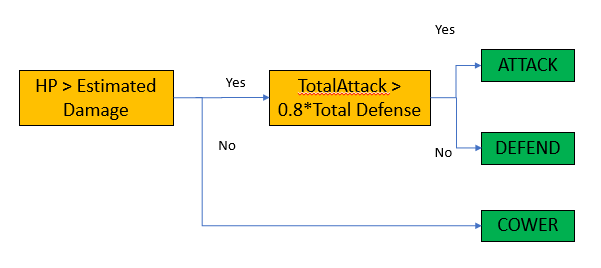
\includegraphics[width=0.5\textwidth]{007_team_4_agent_design/figures/1_fight1.png}
    \caption{Fight decision diagram.}
    \label{fig:fight1}
\end{figure}


\par For the fight manifesto, the threshold of ST and HP being proposed are based on the ratio of agents in each of the quantised categories of ST/HP (low, mid and high ST/HP) - see Equation \ref{eq:1} and Equation \ref{eq:2}. We also calculate a threshold for Attack and Defend points as well, which is simply the average TotalAttack and TotalDefend of all agents.
If the agent's HP or ST are smaller than threshold of HP or ST, this means that it is unwise to fight and so it makes the agent cower. Otherwise, if both HP and ST are above the threshold, the agent must fight. In this case, the agent will attack or defend if its TotalAttack and TotalDefend are greater than the Attack and Defend thresholds, respectively. If the agent is capable of both attacking and defending, this is solved by the server, following the agent's fight decision.

\begin{equation}  
thresholdHP = N_{LowHP}*(250) + N_{MidHP}*(500) + N_{HighHP}*(750)
\label{eq:1}
\end{equation}

\begin{equation}  
thresholdST = N_{LowST}*(500) + N_{MidST}*(1000) + N_{HighST}*(1500)
\label{eq:2}
\end{equation}

\par Our agent now may face impasse if our fight decision stand against what we are proposing in the fight manifesto e.g. our manifesto imposes our agent to fight and the fight decision is to cower. Hence, our agent must choose between the social good and a selfish behavior, which is done by altering our proposal for the fight manifesto in order to fit the fight decision (put agent's stats as thresholds). This behaviour is modeled by a random variable with high probability of not being selfish, in order to align with our agent's ideology (economy of esteem). If our agent decide to follow down the selfish path, its social contribution C is decremented. Otherwise, C is incremented. This impasse is represented in Figure \ref{fig:impasse}.

\begin{figure}
    \centering
    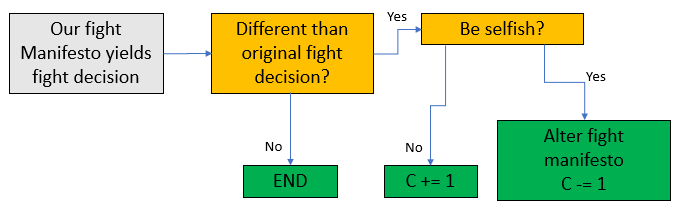
\includegraphics[width=0.5\textwidth]{007_team_4_agent_design/figures/2_fight2.png}
    \caption{Fight decision impasse diagram.}
    \label{fig:impasse}
\end{figure}

\par Next, we also perform voting on the fight manifesto broadcasted by the chair. Logically, our agent wants a manifesto that is similar to its proposal. 
Hence, a tolerance interval is defined for every attribute in the manifesto and if all the HP, ST, TotalAttack and TotalDefend values proposed fall within a certain range (the certain range is calculated based on our proposed values in our manifesto and the tolerance),  we vote “YES”, as this indicates a high similarity with our proposed manifesto. Otherwise, we vote “No”. 

\par After establishing a social contract on fighting decisions, we may decide to obey it or disobey it. The latter is only chosen if our agent's HP or ST are in a critical level and we are told to fight. If the two actions decided from our own heuristic and voted manifesto are not the same and we choose to obey the social contract, our C is incremented since we did something for greater common good. On the other hand, if we disobey, our C is decremented.
 

\par With these two ideas, our agent try to maximize social contribution and survive at the same time.

\par As mentioned in section 7.1, we also monitor agent's social contribution. When an agent attacks or defends with low HP or ST, it is prioritizing the common good and because of that its social contribution value is incremented. On the other hand, when an agent cowers with both high HP and ST it is prioritizing its own interests and hence, its social contribution value is incremented. This information will be used for trading and voting for a chair.

\section{Post-combat}

\par There are several actions we can perform during the post-combat round, which are donating HP to the health pool, trading with other agents, distributing loots, electing/deposing chair and handling disobedience.

\subsection{Donating HP to the Health Pool}

\par By donating HP to the health pool, we may be able to skip the combat round hence all other agents do not need to fight and take damage. This is beneficial to everyone. Therefore, if our HP is greater than a certain percentage of our total HP and our social contribution C is below a certain threshold (this means we are not contributing enough to the common good), we will donate a fraction of our HP (10\%) to the health pool. As a result, we increase our social contribution to indicate we have contributed to the common good. 

\subsection{Trading}

\par For trading, we are going describe our strategies on how to make requests to other agents and respond requests from other agents. We further separate the logic for each item (Weapon and Shield). Moreover, we assume that we always keep the best weapon and shield for ourselves so that we can maximize the damage we can deal and minimize the damage we may take. 

\par For making requests on weapon, if our TotalAttack is smaller than ST, then we ask for a better weapon from other agents so we can maximize the damage that we can deal.

\par For making requests on shield, if our TotalDefend is smaller than ST, then we ask for a better shield from other agents so we can minimize the damage that we may receive.

\par For responding requests, we will accept requests more frequently if we have more items in the inventory so we are not going to waste resources and maximize the common good. If our social contribution is negative (this means that we rarely contribute to the common good), we always accept requests no matter what the requests are, and then increase our social contribution. However, if our social contribution is positive, we further decide whether we should trade based on how many items we have and a trading threshold. If the result of dividing the number of items by our social contribution (Equation \ref{eq:3}) is lower than the trading threshold, we are not going to trade. Otherwise, we will accept the requests. In Equation \ref{eq:3}, we divide by C so that if C is high, we have smaller number and hence we don't always trade.

\begin{equation}  
tradeEval = (N_{swords} + N_{shields}) / C
\label{eq:3}
\end{equation}

\par In addition, we also consider social contributions of other agents when trading. When requesting items, we prioritize agents with higher social contribution since there is a higher chance the trade will be successful. We only accept requests from agent whose social contribution is acceptable (e.g. higher than -4) and their disobedience value is not zero (see Section 7.3.5).

\par Finally, for successful trades, we increment the respective agent's social contribution. Figures \ref{fig:trademake} and \ref{fig:traderec} show the flowcharts for making and receiving requests, respectively.

\begin{figure}
    \centering
    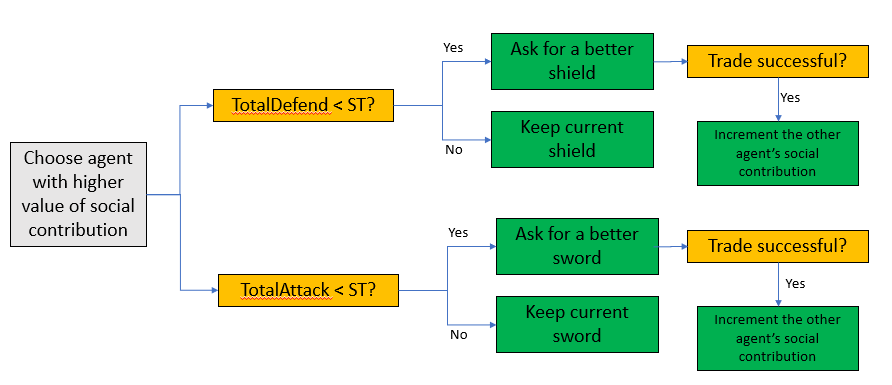
\includegraphics[width=0.5\textwidth]{007_team_4_agent_design/figures/4_trading_make.png}
    \caption{Trading structure for making requests.}
    \label{fig:trademake}
\end{figure}

\begin{figure}
    \centering
    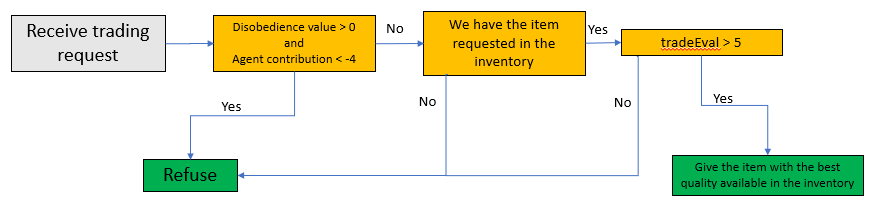
\includegraphics[width=0.5\textwidth]{007_team_4_agent_design/figures/3_trading_receive_2.png}
    \caption{Trading structure for receiving requests.}
    \label{fig:traderec}
\end{figure}

\subsection{Loot Distribution}

\par For the loot manifesto, the threshold of ST, HP, Attack and Defend are estimated with the same idea in the fight manifesto. If the agent's HP is smaller than the HP threshold (Equation \ref{eq:1}), it is allowed to get a HP potion from the loot pool if there is one. Similarly, if its ST is smaller than the ST threshold (Equation \ref{eq:2}), the agent is allowed to get a ST potion from the loot pool if there is one. Also, if both our HP and ST are greater than the HP and ST threshold, this means that our condition is good enough to fight and we should be equipped for that. Hence, we further analyse the TotalAttack and TotalDefend. If the TotalAttack is smaller than an Attack threshold, then the agent are allowed to get a sword from the loot pool in order to maximize the damage dealt to the monster. Similarly, if its TotalDefend is smaller than the Defend threshold, then then we are allowed to get a shield from the loot pool. We utilize the same voting mechanism in fight manifesto for the loot manifesto.

\par Last but not least, we are allowed to disobey the voted loot manifesto. If our HP is extremely low but our manifesto decision does not allocate us  getting a HP potion even there is one, we can simply get the HP potion and decrease our C at the same time. This case applies to ST potions as well. Figures \ref{fig:lootdist} show the flowchart for deciding which item to get from the loot pool.

\begin{figure}
    \centering
    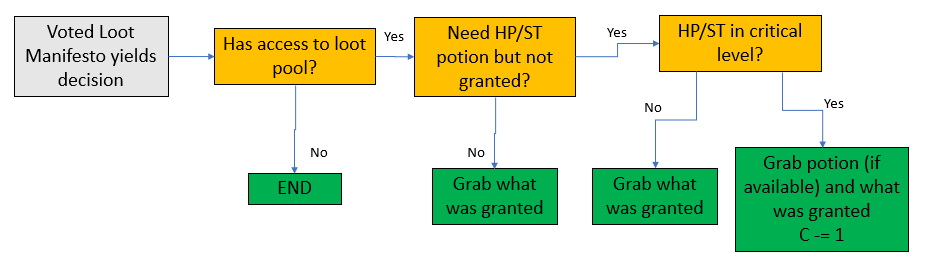
\includegraphics[width=0.5\textwidth]{007_team_4_agent_design/figures/5_loot.png}
    \caption{Structure for loot distribution.}
    \label{fig:lootdist}
\end{figure}

\subsection{Voting for Chair and Deposing}

\par The chair is voted in a simiFlar way that our agent votes for the manifestos and attempts to elect an agent that has a high social contribution rating and a similar governance plan than ours. Hence, if the candidate has (1) less or equal term length (2) similar number of necessary votes to depose (3) loot imposition (4) fight imposition and (5) a positive value of social contribution, we consider voting for that agent. If there is a tie, we will vote for the agent with the highest social contribution value (including our own agent).

\par As for deposing a chair, we analyse the ultimate result of this agent's administration that is, the number of agents killed during its term. If the number of agents alive have decreased 60\% since its election, we vote "YES" for deposing this agent from the chair. If the chair is deposed, its social contribution is decremented.



\subsection{Handling Disobedience}

\par The penalty for disobedience is to refuse all trading requests for a some period of time. Technically, each time an agent disobey, its disobedience value is incremented, and at the end of every 3 rounds, this value is decremented. This creates a mechanism of punishment by locking away those agents from trading with our agent. For instance, if an agent disobey the social contract, we don't accept trade requests with that agent for 3 rounds (until the disobedience value is decremented to 0). This also has a cumulative effect, so if an agent disobey twice in the same round, it gets a 6-round punishment, which may reinforce the importance of trusting the institution in power and and following social contracts. 

\section{Governance}
\par Our chair campaigns with the following manifesto: Number of levels - 10, Percentage of votes to depose: 65, Fight Imposition - Yes, Loot Imposition - Yes. Based on our governance strategy below, the actions of the agents may require a few levels to reach the ideal results, as such our agent is campaigning to be in power for many levels. However, in the event that most agents do not want a chair for too long, we capped his/her term at 10 levels. The decisions to utilize a fight and loot imposition will be discussed below.
 
 \par The focus behind creating an apt system of governance, is how the knowledge of this elected chair is managed. Our governance is primarily based on an economy of esteem, which is a system that rewards agents who act in a manner that contributes to the progress of the group. This contribution is recognized in the form of attacking and defending, and the reward is in the form of a greater influence in voting on a proposal regarding fight and loot decisions. This is based upon the Athenian system of government in which greater cooperation and contribution to the collective resulted in greater social benefits. Our chair aggregates knowledge based on prior fight actions; we chose 3 prior rounds as this was long enough to assess patterns in agents’ behaviour but not so long as to prevent an agent from being able to change behaviour. Upon having the proposals from each agent, a weighted mean is taken of the thresholds for attacking, defending, and loot acquisitions, creating a new proposal. The weights of this mean are the number of votes an agent can have. Having fought (attacked or defended) 3 times in the past 3 rounds, gives an agent 4 votes, having fought twice gives 3 votes, having fought once gives 2 votes, and having fought 0 times gives 1 vote. The benefit of this approach is two-fold. Firstly, it incentivizes agents to contribute more to the collective good by rewarding them with a greater ability to make a choice. Secondly, given that an agent who has been fighting in the past few rounds has lower health, it gives them a greater voice to explain why they potentially deserve to rest in the form a cower decision. Once this new weighted proposal is created it is broadcasted to all agents to vote on it. If the vote does not pass, the weight of each category is decremented by one, except those of agents who did not fight at all in the past 3 rounds. This yields a proposal closer to the simple majority and then is broadcasted again, and the process repeats each time a vote does not pass. While simple majorities are not the best form of knowledge aggregation, the voting not passing multiple times suggests that the desire of the agents is closer to a simple majority than a weighted mean based around the collective good. As a result of creating and broadcasting a new proposal, our leader requires both the fight imposition and loot imposition.

\par Even in the case of a vote passing, certain agents are bound to be disobedient. Based on Ostrom’s 5th principle, there must be sanctions for those who disobey their expected action. However, our chair is not completely ruthless and is aware that very harsh punishments cause punished agents to resent the governance and the overall institution. As such, our chair only imposes sanctions in the form of reputation consequences by broadcasting, when an agent has disobeyed their assigned task, and how many times that agent has disobeyed. It is ultimately, up to each individual agent to decide how they want to deal with agents who disobey the chair.  

\section{Experiments and Discussion}


Experiment 1:
The first experiment was to analyze the performance of the game using set parameters. The parameters were 60 levels, starting health points of 1000, starting attack of 20, starting shield of 20, base stamina of 2000 and a threshold that 60\% of the agents must survive.
Figure \ref{fig:exp1results} shows the results obtained by setting these parameters in the .env file of the repository. 

We can see that for the number of agents remaining at the end of each level, the line becomes quite consistent up to level 20. This means that we have 100 agents up to level 20 which shows strong performance under our agent strategy. The same pattern can be seen with the number of agents remaining at the end of each round. Up until round 67, the consistency of the line is very high showing that 100 agents have remained until round 67. However, it slowly starts to decline after this point where round 85 is left with 55 agents (game lost). 

The HP pool graph shows interesting trends where we see the HP pool gravitate upwards to 20,000 on level 4 (the maximum peak). However, it decreases after this point with no rise which indicates that agents stopped donating to the HP pool, and by level 16 the agents start to constantly having to fight, which leads to a loss in the game.

\newpage
\begin{figure}[htbp]
\begin{tabular}{ll}
    \centering
    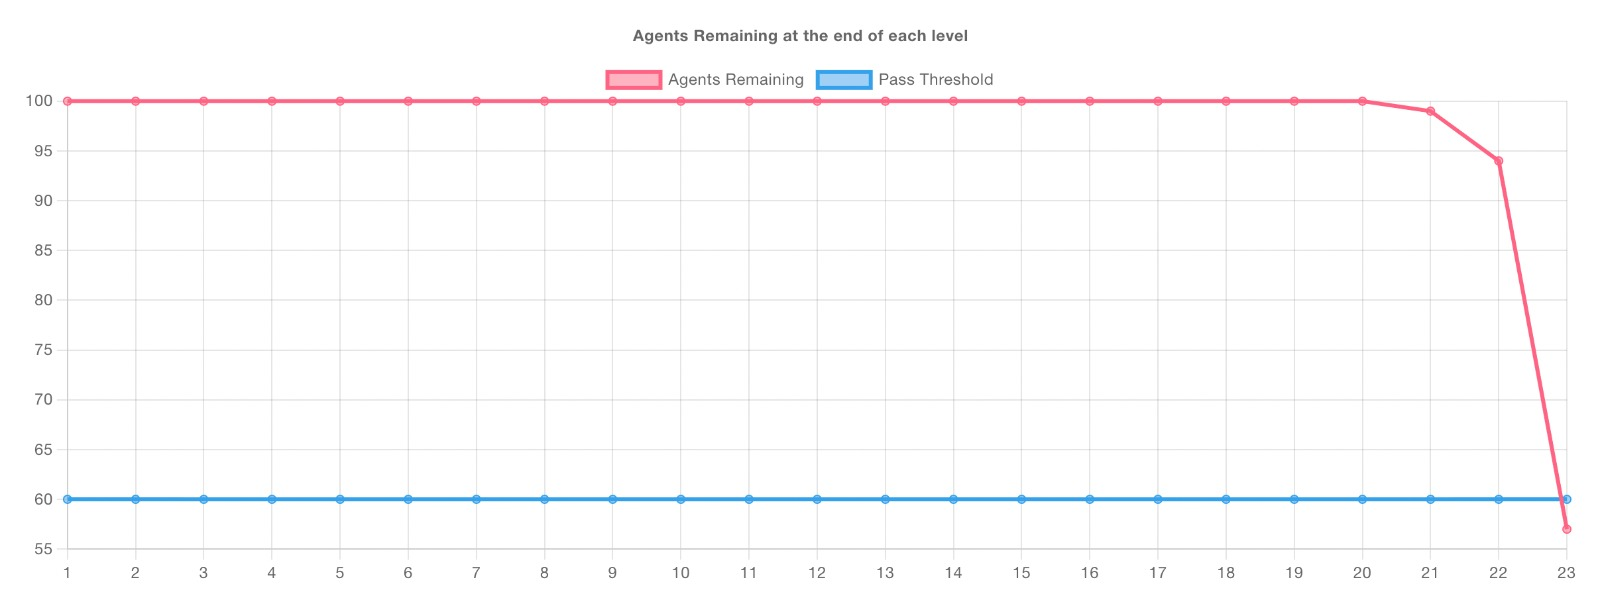
\includegraphics[width=0.5\textwidth]{007_team_4_agent_design/figures/EX1_1.jpg}
    &
    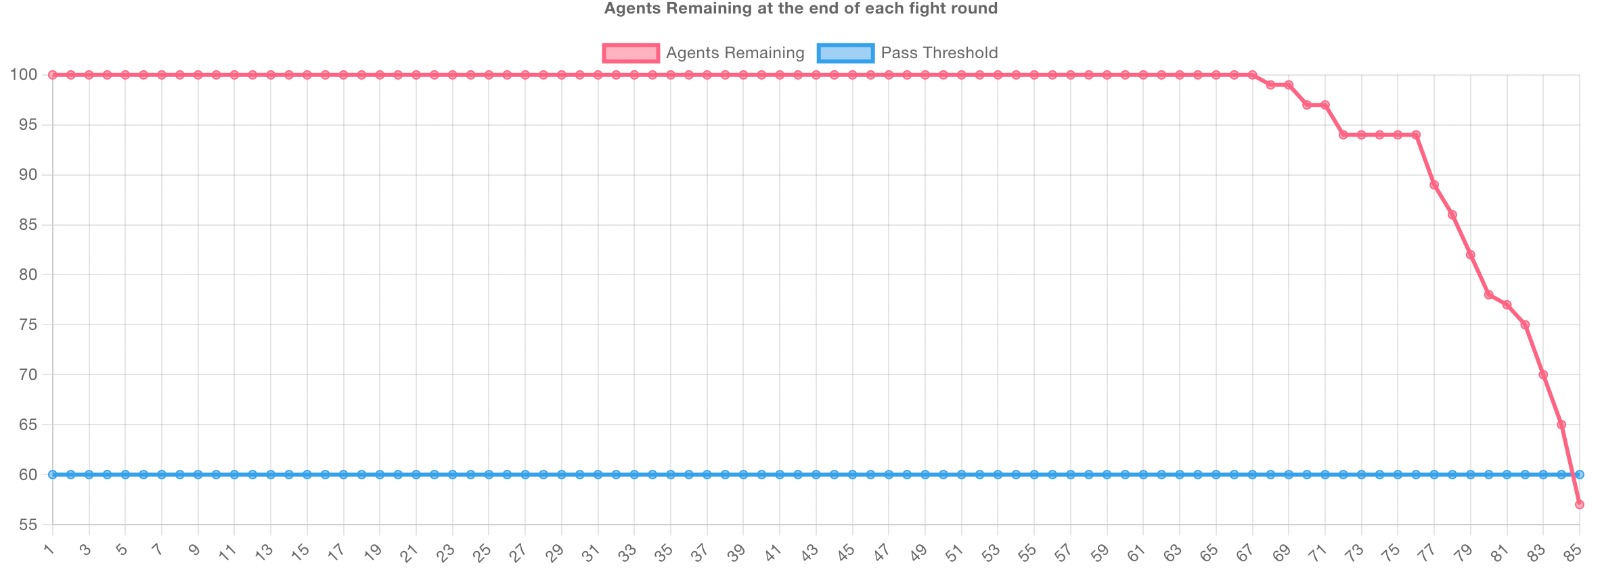
\includegraphics[width=0.5\textwidth]{007_team_4_agent_design/figures/EX1_2.jpg}
\end{tabular}

\end{figure}

\begin{figure}[htbp]
\begin{tabular}{ll}
    \centering
    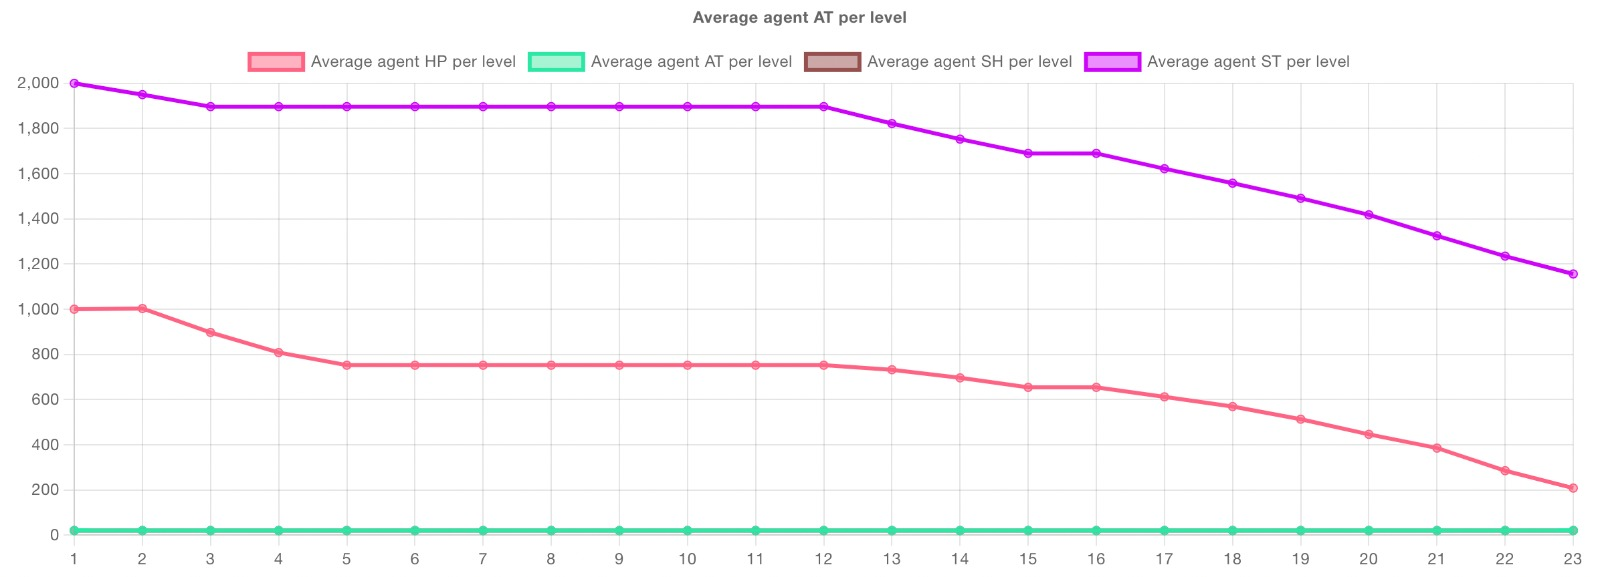
\includegraphics[width=0.5\textwidth]{007_team_4_agent_design/figures/EX1_3.jpg}
    &
    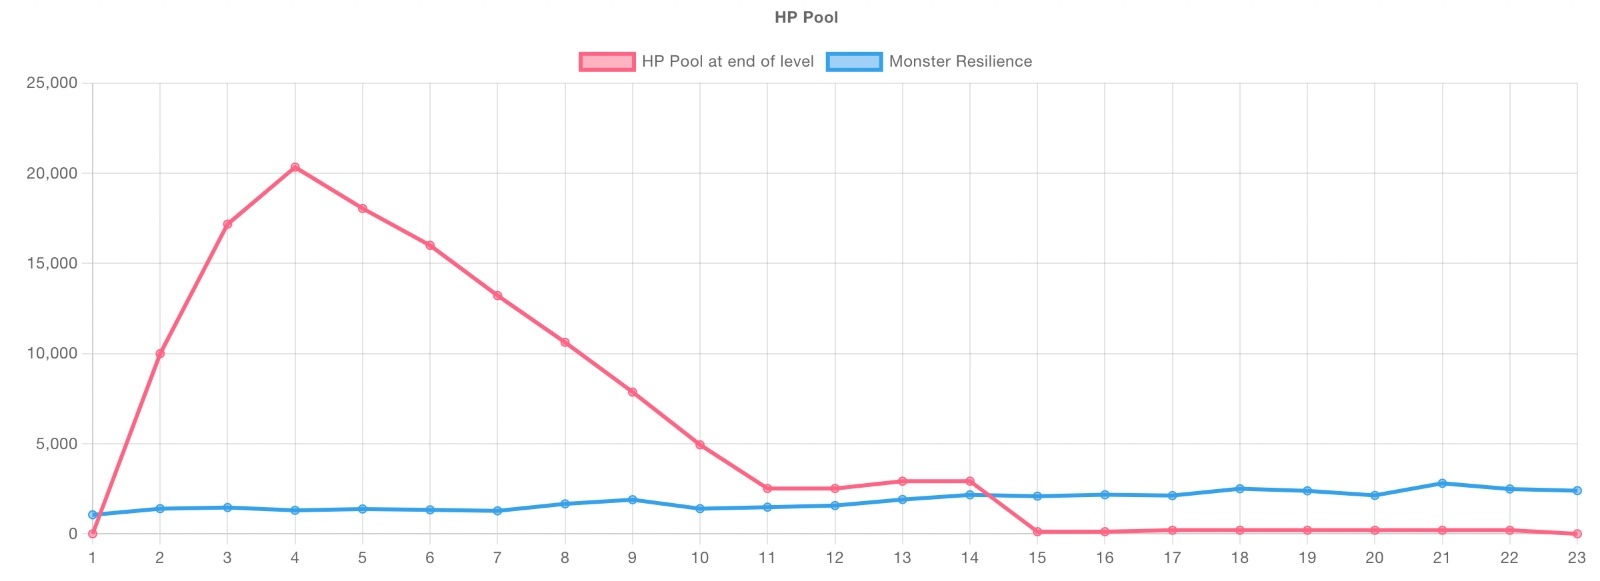
\includegraphics[width=0.5\textwidth]{007_team_4_agent_design/figures/EX1_4.jpg}
\end{tabular}
     
\end{figure}


\begin{figure}[htbp]
\begin{tabular}{ll}
    \centering
    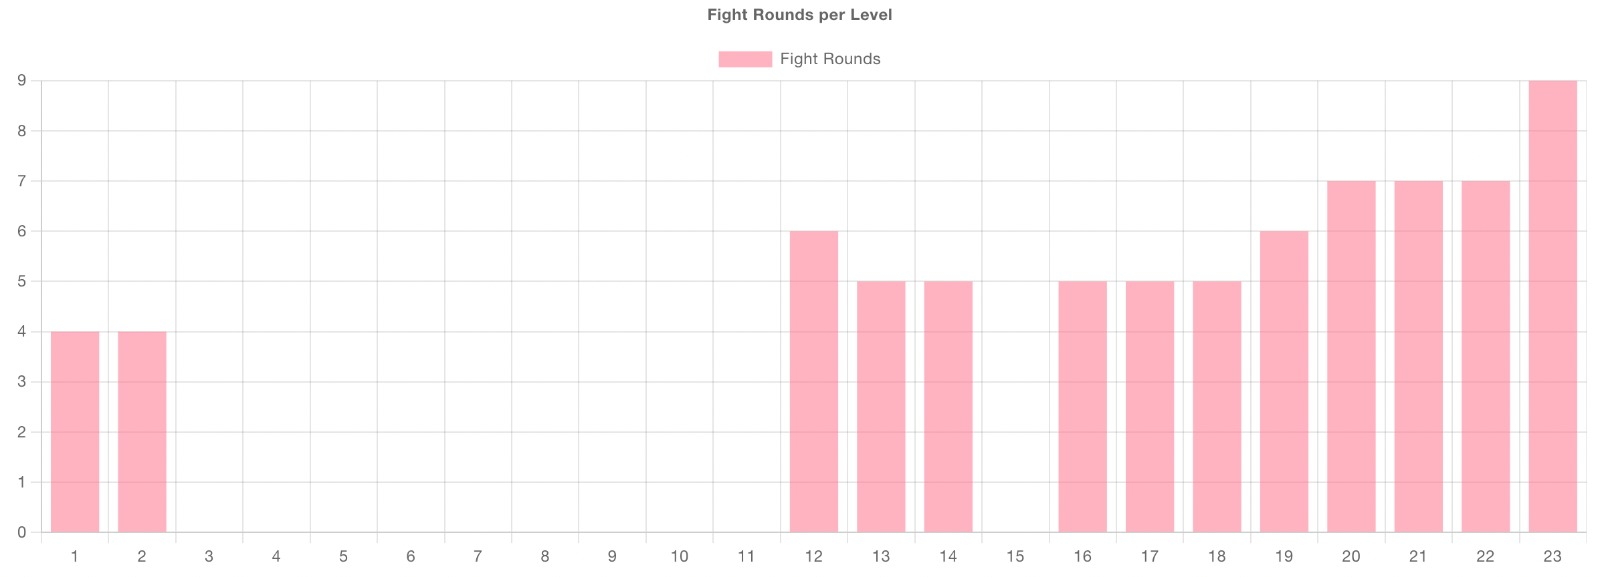
\includegraphics[width=0.5\textwidth]{007_team_4_agent_design/figures/EX1_5.jpg}
    &
    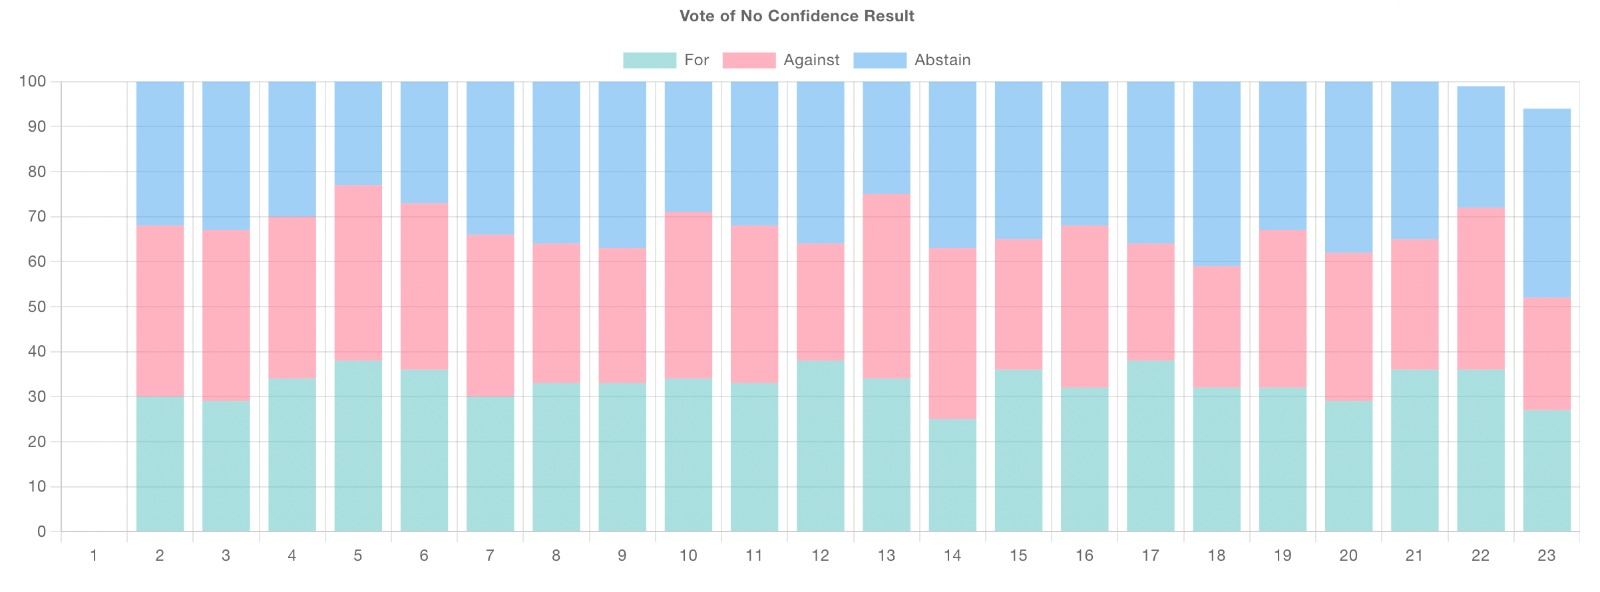
\includegraphics[width=0.5\textwidth]{007_team_4_agent_design/figures/EX1_6.jpg}
\end{tabular}
    \caption{Experiment 1 results}
    \label{fig:exp1results}
\end{figure}

\newpage

Experiment 2:
\par The parameters were now changed from 60 to 20 levels from the first experiment. Figure \ref{fig:exp2results} shows the results obtained by setting these parameters in the .env file of the repository. 

The first two graphs depict the number of agents remaining at the end of each level or fight round. The pass threshold is set at 60, meaning that a minimum of 60 agents are required to progress. The graphs show that the number of agents begins to decline at round 23, and around mid 25, the number of agents falls to the pass threshold. After this point, the number of agents significantly decreases.

The HP pool graph shows the fluctuations in the total health of the agents over time. At level 2, the HP pool reaches its highest point at around 1,500. After this, the pool decreases and does not increase again, indicating that agents have stopped contributing to the pool. Differently from Experiment 1, we can see that the number of agents donating to the HP pool is not sufficient in the first level, so they must fight right at the beginning of the game, and are not able to scavenge good loot. Hence, they cannot handle the monster and lose the game in the next couple of levels.  


\begin{figure}[htbp]
\begin{tabular}{ll}
    \centering
    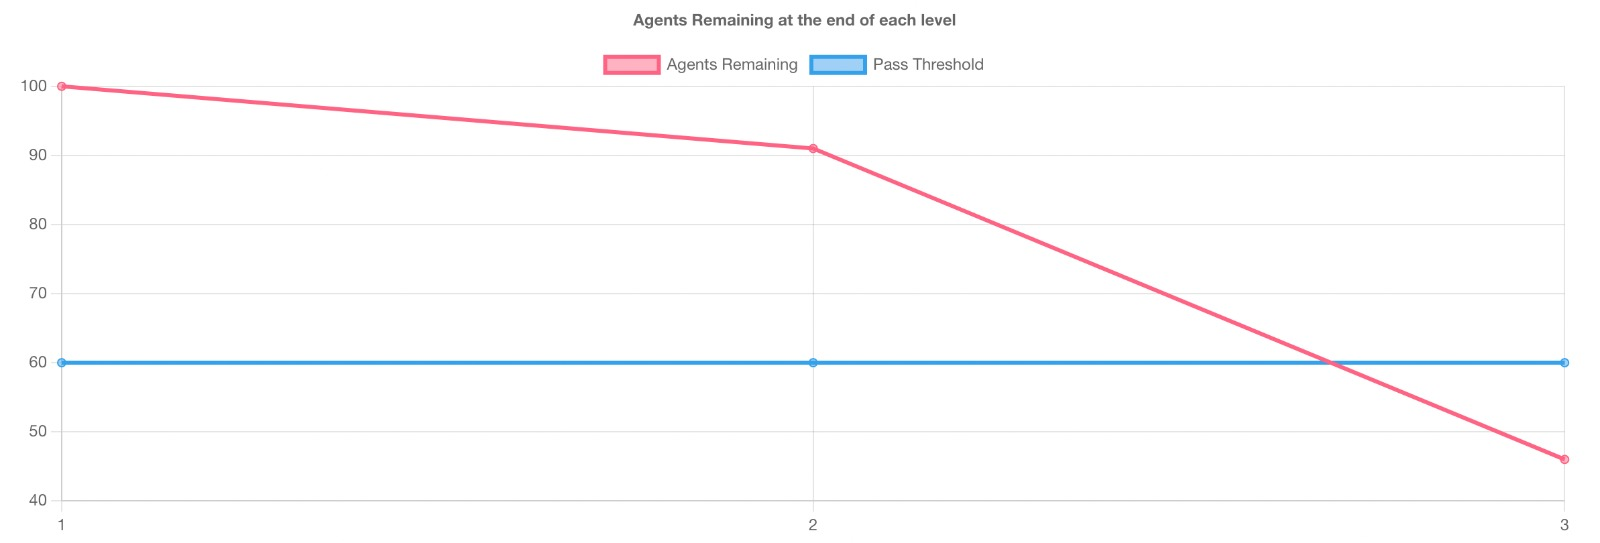
\includegraphics[width=0.5\textwidth]{007_team_4_agent_design/figures/EX2_1.jpg}
    &
    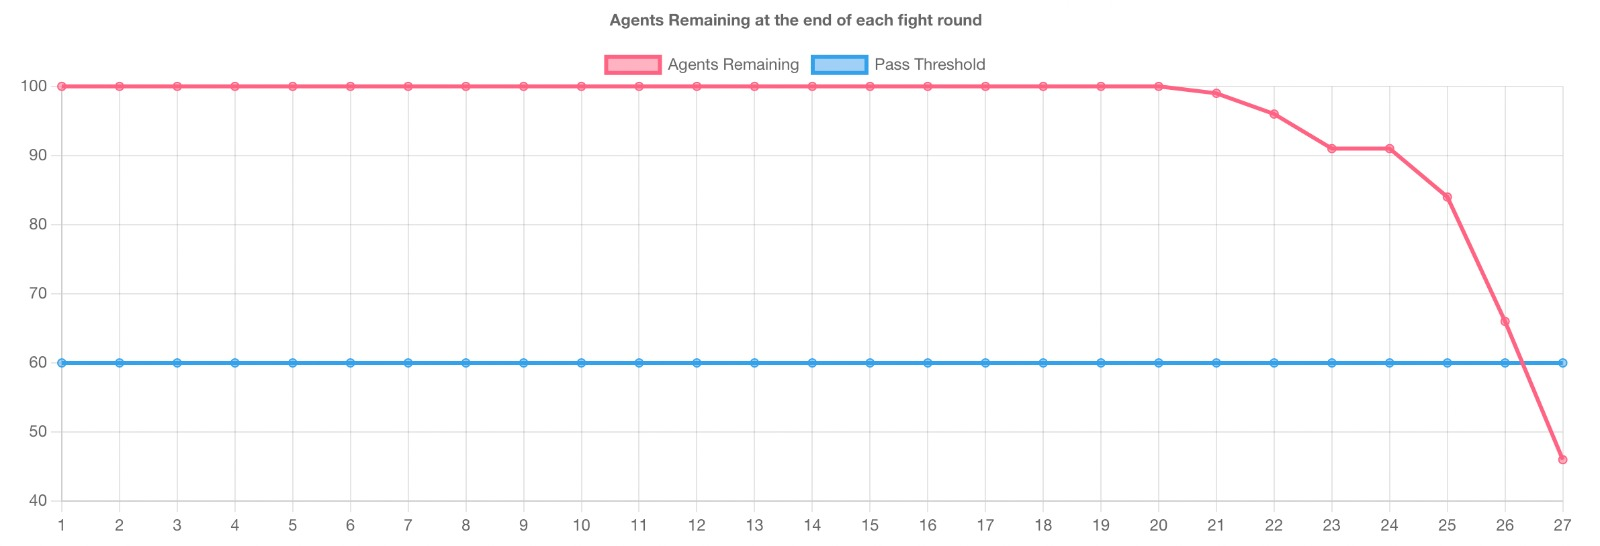
\includegraphics[width=0.5\textwidth]{007_team_4_agent_design/figures/EX2_2.jpg}
\end{tabular}

\end{figure}

\begin{figure}[htbp]
\begin{tabular}{ll}
    \centering
    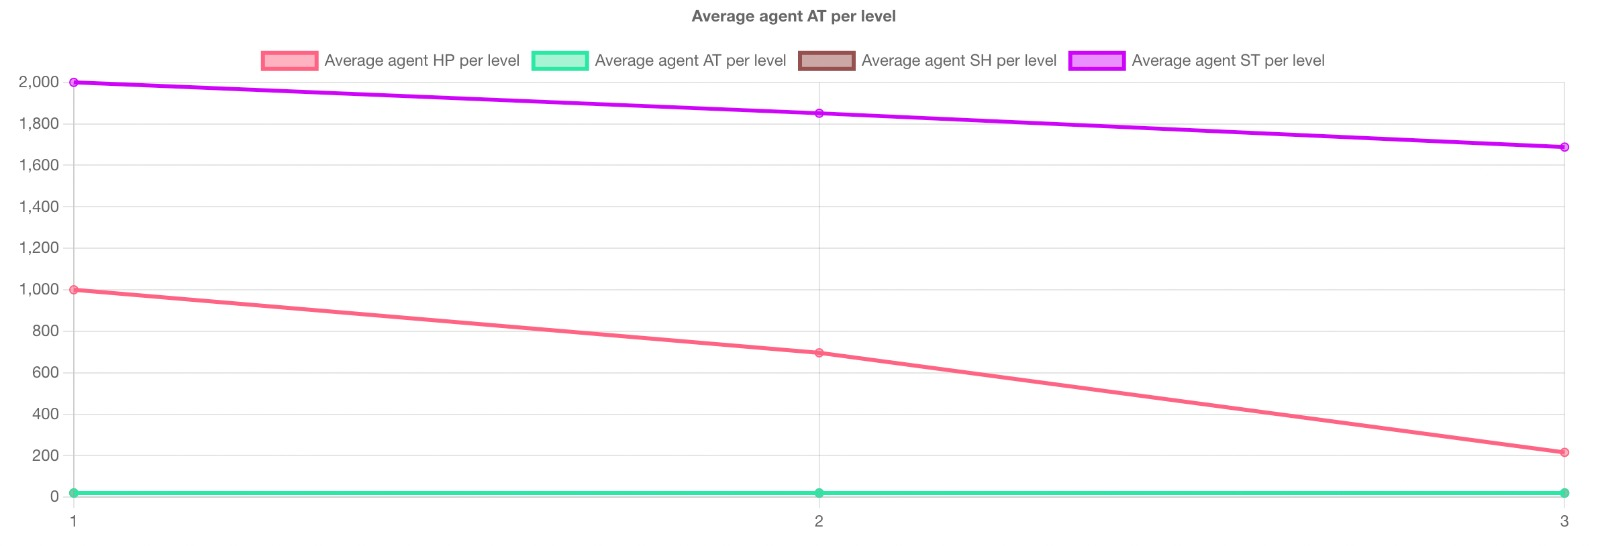
\includegraphics[width=0.5\textwidth]{007_team_4_agent_design/figures/EX2_5.jpg}
    &
    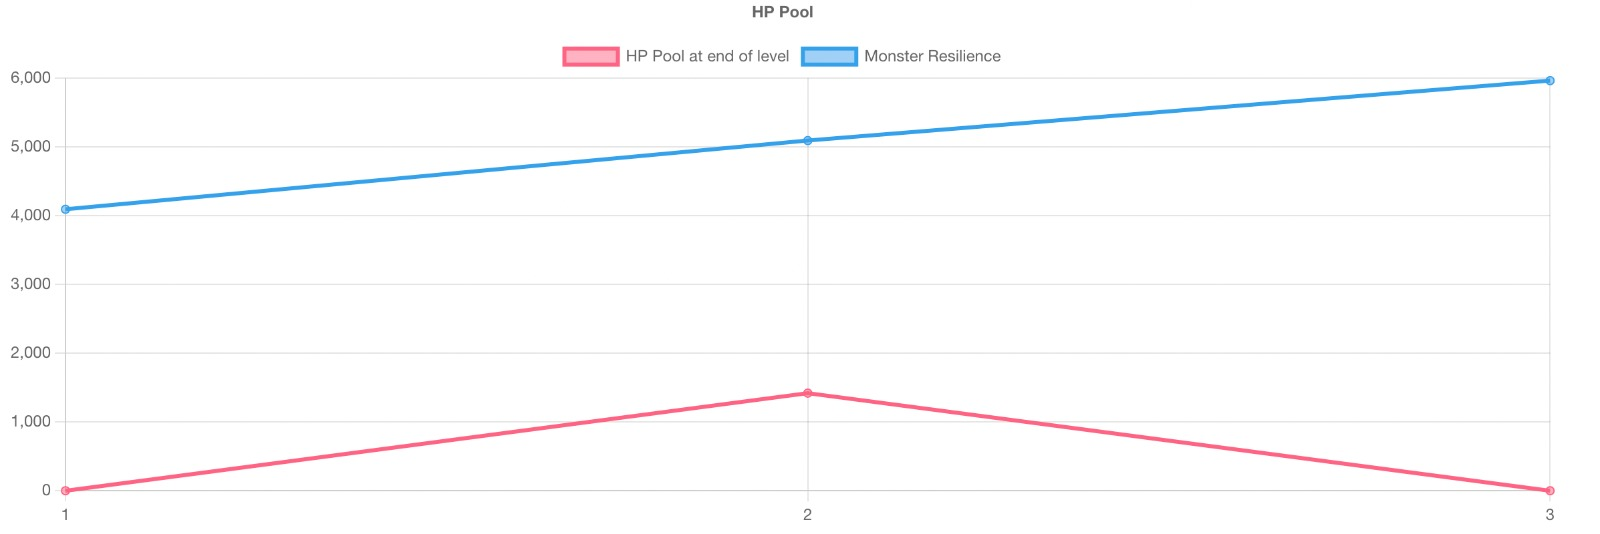
\includegraphics[width=0.5\textwidth]{007_team_4_agent_design/figures/EX2_6.jpg}
\end{tabular}

\end{figure}


\begin{figure}[htbp]
\begin{tabular}{ll}
    \centering
    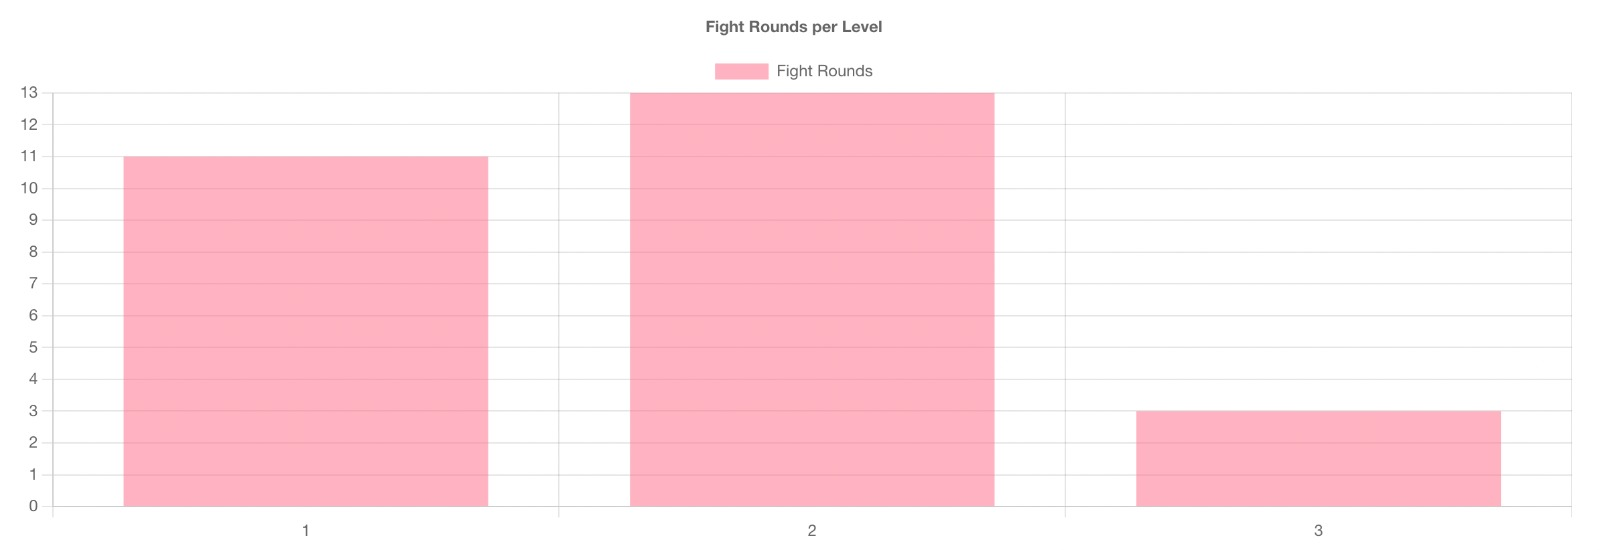
\includegraphics[width=0.5\textwidth]{007_team_4_agent_design/figures/EX2_3.jpg}
    &
    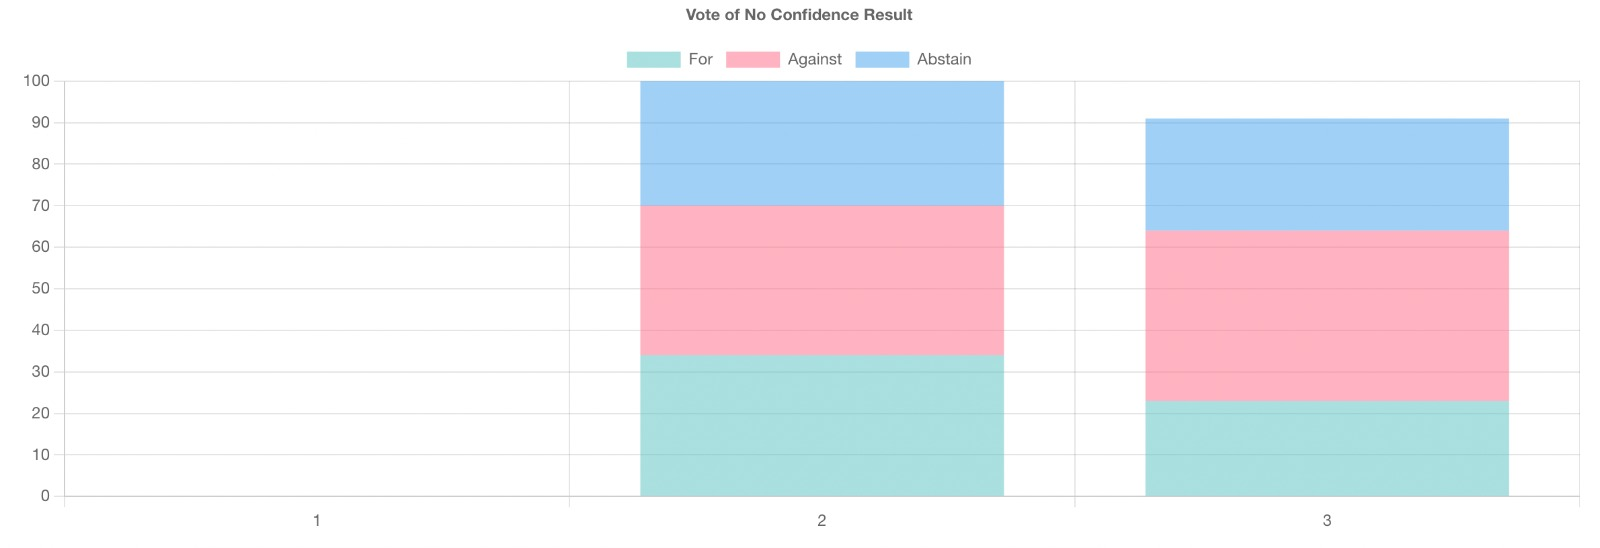
\includegraphics[width=0.5\textwidth]{007_team_4_agent_design/figures/EX2_4.jpg}
\end{tabular}
    \caption{Experiment 2 results.}
    \label{fig:exp2results}
\end{figure}


\newpage

Experiment 3: The parameters were now changed so that there are only 30 of our agent in the game. Figure \ref{fig:exp3results} shows the results obtained by setting these parameters in the .env file of the repository. 

\par The first two graph shows the number of agents remaining at the end of each level or fight round. The pass threshold is set at 18, meaning that the minimum number of agents required is 18. Initially, the number of agents remaining is 30, but as the levels progress, the number of agents significantly declines and reaches its minimum at level 25 (or round 97).

The HP pool graph displays the trends in the HP pool, with similar behavior as in Experiment 1. At level 4, the HP pool reaches its maximum peak of 7,000. However, after this point, the HP pool decreases and does not rise again, indicating that agents may have stopped contributing to the pool. From level 12 onwards, the agents appear to constantly be in fights, as indicated by the constant decrease in the HP pool.


\begin{figure}[htbp]
\begin{tabular}{ll}
    \centering
    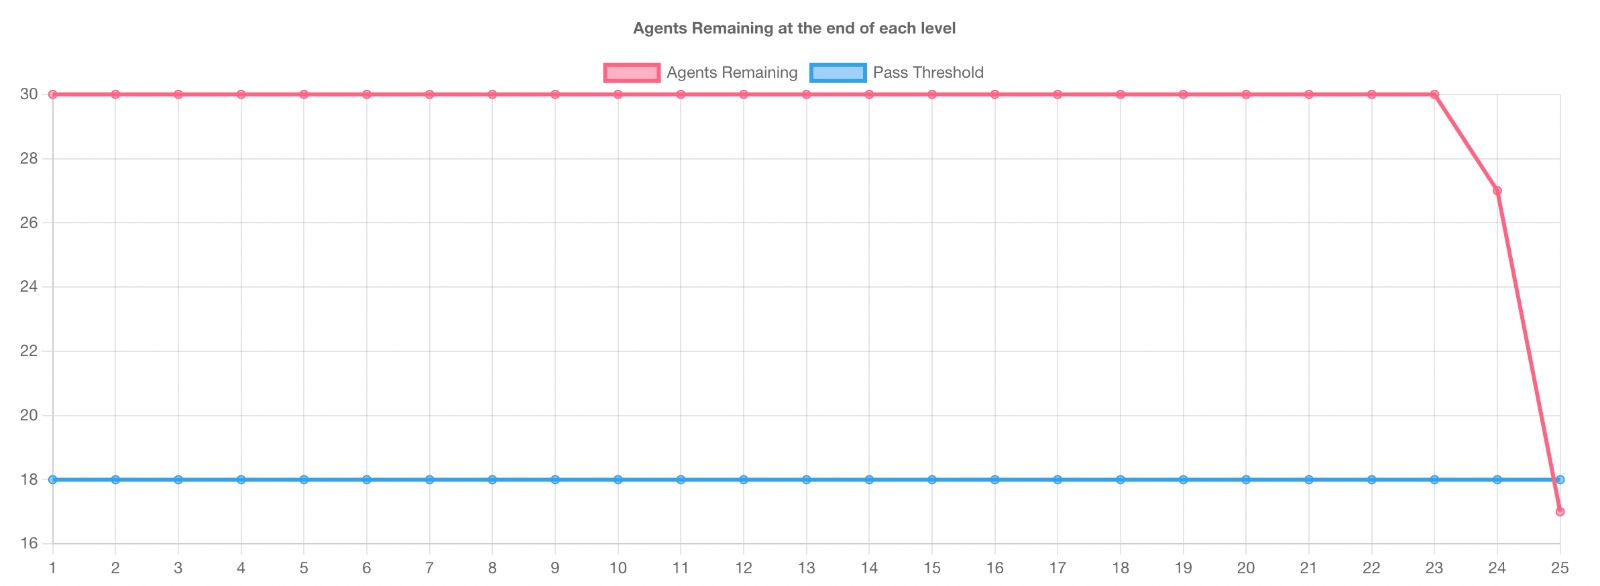
\includegraphics[width=0.5\textwidth]{007_team_4_agent_design/figures/EX3_1.jpg}
    &
    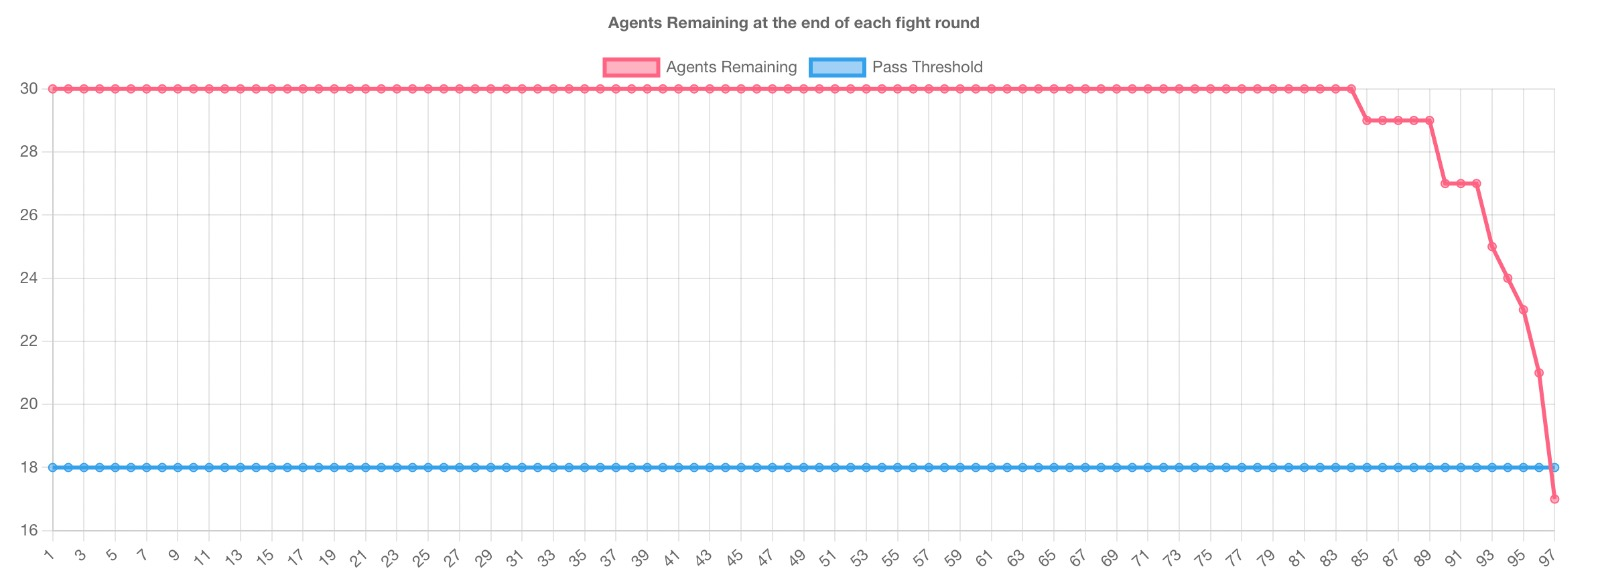
\includegraphics[width=0.5\textwidth]{007_team_4_agent_design/figures/EX3_2.jpg}
\end{tabular}

\end{figure}

\begin{figure}[htbp]
\begin{tabular}{ll}
    \centering
    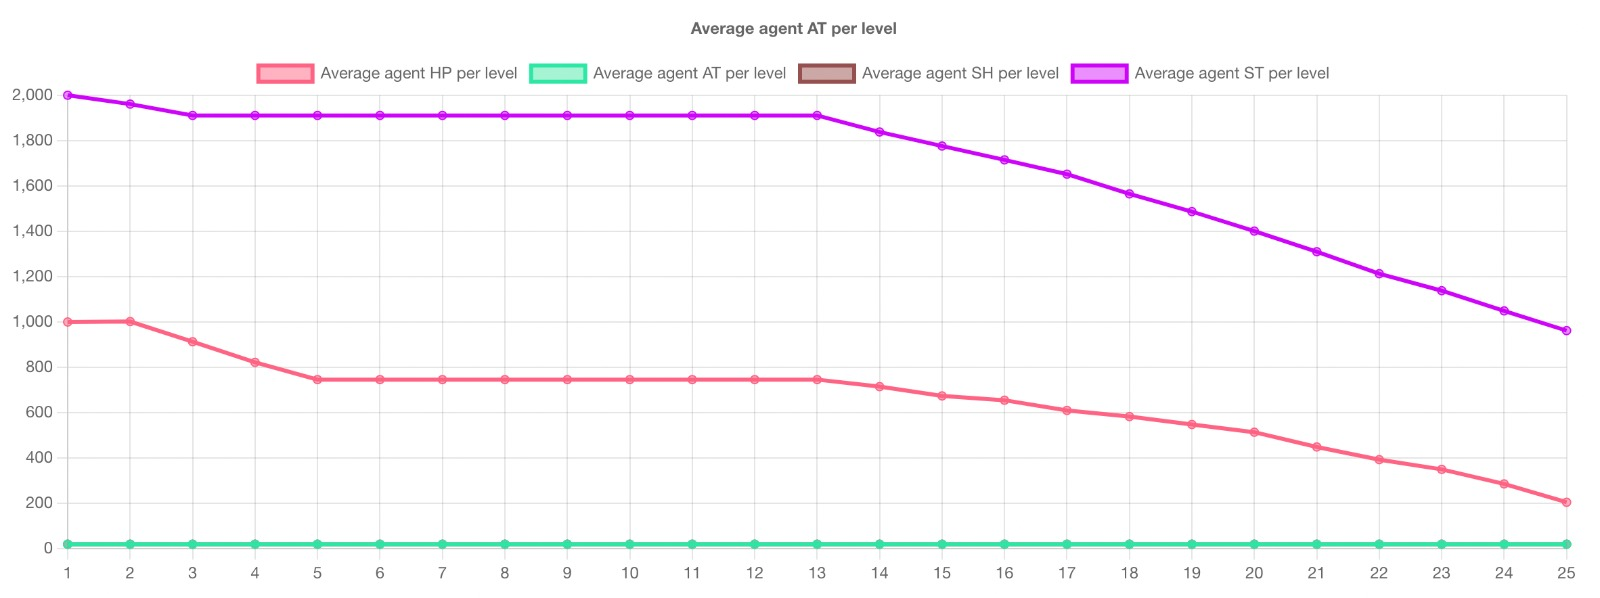
\includegraphics[width=0.5\textwidth]{007_team_4_agent_design/figures/EX3_3.jpg}
    &
    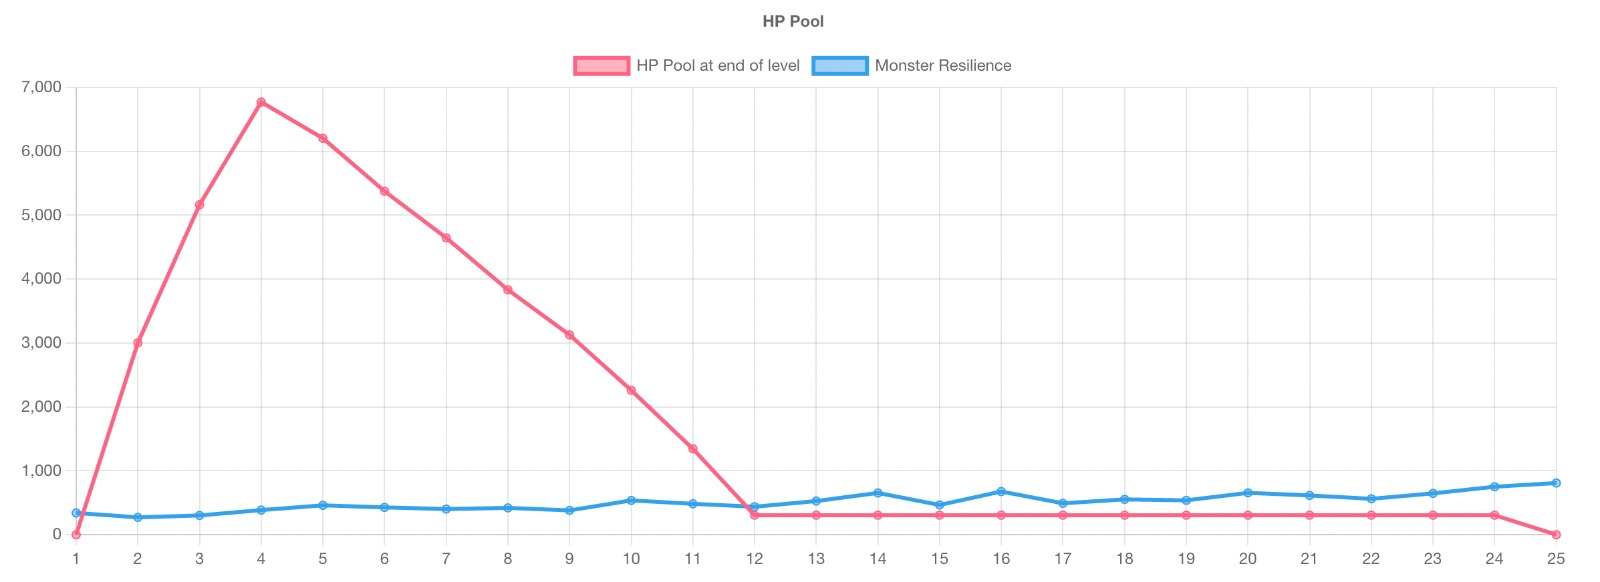
\includegraphics[width=0.5\textwidth]{007_team_4_agent_design/figures/EX3_4.jpg}
\end{tabular}

\end{figure}


\begin{figure}[htbp]
\begin{tabular}{ll}
    \centering
    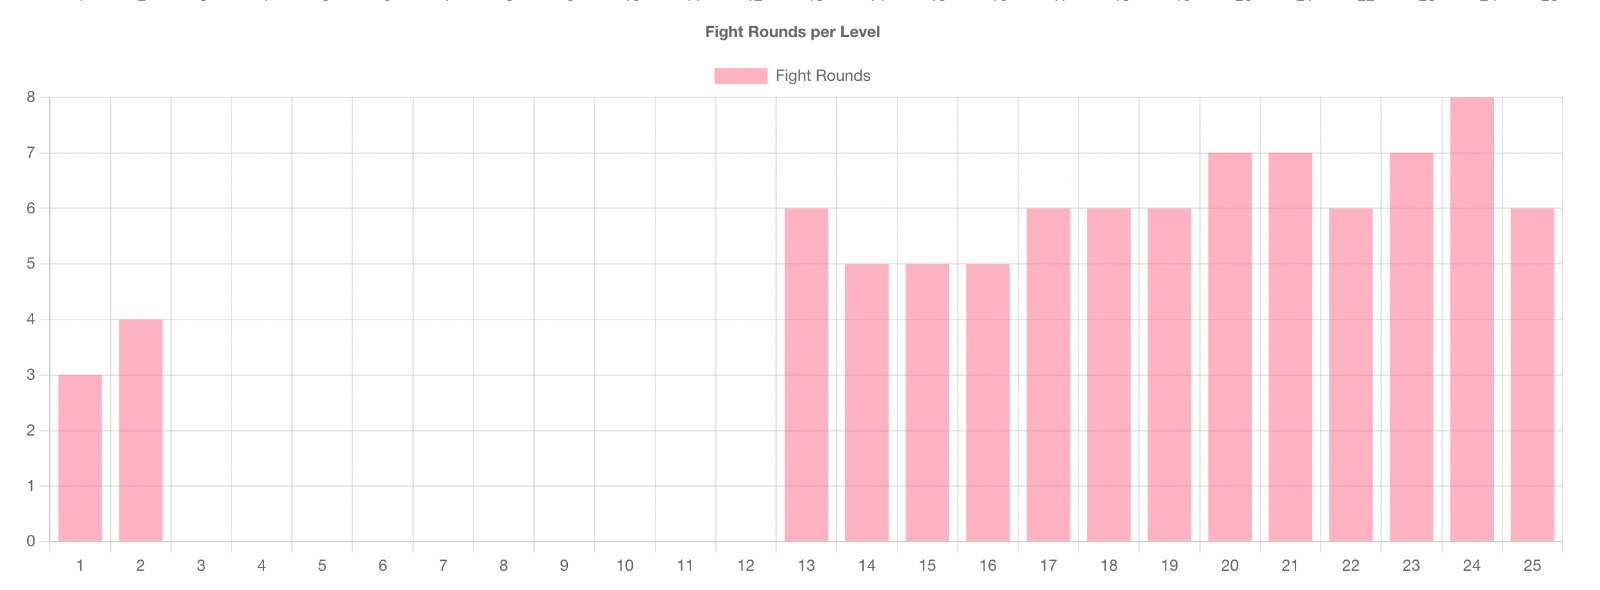
\includegraphics[width=0.5\textwidth]{007_team_4_agent_design/figures/EX3_6.jpg}
    &
    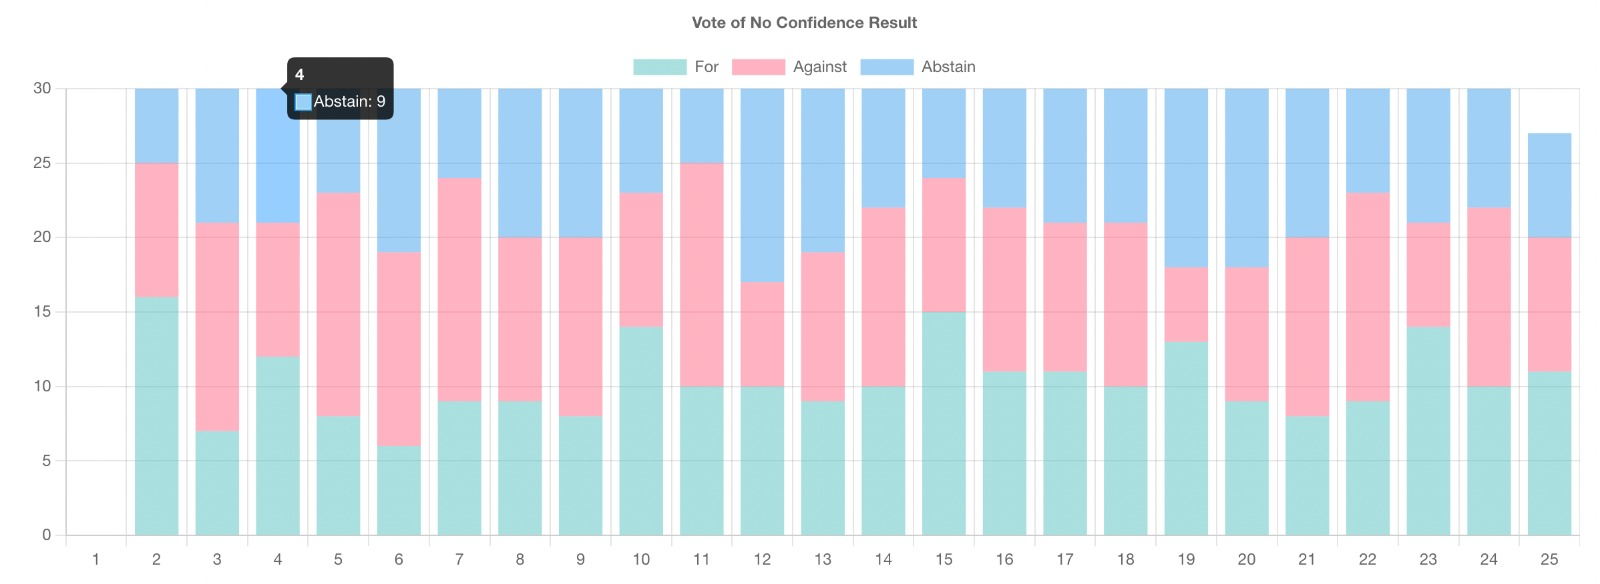
\includegraphics[width=0.5\textwidth]{007_team_4_agent_design/figures/EX3_5.jpg}
\end{tabular}
    \caption{Experiment 3 results.}
    \label{fig:exp3results}
\end{figure}


\par In all the experiments, the agents lost and couldn't escape the pit. It was observed that the agents tend to donate to the HP pool, and this strategy works for a limited time, since the average HP seems to be constantly decreasing. This may happen due to a lack of health potions dropped by the monster, or a poor loot allocation. Furthermore, when agents start to have to fight, it is in fact observed that they manage to survive and maintain a good performance for some levels, until the difficulty is increased to a very high intensity, which cannot be handled by the agents.


\newpage

\par Given our agent operates under an economy of esteem, it's key idea is to ensure that it balances social contributions with its chances of survival. For instance, when reaching an impasse with the fight decision, our agent follows the logical decision for the common good more frequently. Also, it chooses to interact/trade with agents with a higher social contribution value and do not disobey social contracts, which reinforces the ideology implemented. Also, by donating to the HP pool, we can see how beneficial it was in the simulations, since as soon as the agents start fighting the monster, they start to encounter difficulties and were not able to win the game. This reveals that contribution to social good yields better results than a selfish mindset. At the same time, the variable C balances the amount of our agent's social contributions, so that it doesn't always choose to contribute to the social good and makes it prioritize its own survival.

\par By analysing the experiments 1 and 3 (60 levels) we can notice that our agent performs better than the random agent (survives until level 18). One of the reasons for that is our agent takes into consideration past actions from other agents in order to make a decision. With this learning process, our agent surpasses the random agent performance by replacing randomness for knowledge when making a decision. Also, in our agent's strategy, for the fight manifesto, the majority of agents fighting will be attacking since too many agents defending may lead to a prolonged level and a lot of damage being taken. Furthermore, our manifesto for loot distribution is based on each agent's current needs, which is an attempt to optimise the stats for each agent before the new level starts. Finally, we have a governance ideology that rewards agents that contribute to the social good, giving them more importance in voting.


\par It is valid to mention that our initial strategy included interactions with other agents before deciding our fight action. Essentially, it would ask other agents for their actions and take their responses into consideration to estimate how many agents would fight or cower. Unfortunately, this was not implemented since the infrastructure to make this communication possible was not completed. Therefore, the agent strategy that we wanted to implement was based on pre-fight communications which consisted on storing all the agent fight decisions (not just manifesto decisions) from the beginning to the end of the game. This would allow our agent to use predictive learning to past actions as a method to predict future actions which would optimize our chances of choosing better actions through prediction. Based on a given condition, the action of that particular agent would be stored until it iteratively goes through each agent action until the game is done.

\section{Future Steps}

\par Given the opportunity to better our agent, there are a few changes we would make to its design. One is the existence of a clear reputation framework. While different agents have abilities to assess their opinions of agents in the form of the social contribution (C), the existence of a standardized framework in which all agents can express their opinions on other agents and send these views to the chair would allow for a more robust economy of esteem. This would allow agents to make connections with other agents, and identify their reputation based on their fight decisions, amounts of trading, and interactions with other agents. The weights of these connections would change based on how often agents communicated which would relay to the chair how valid an opinion of another agent might be. 

%------------------------------------------------------------------end

